%%%%%%%%%%%%%%%%%%%%%%%%%%%%%%%%%%%%%%%%%%%%%%%%%%%%%%%%%%%%%%%%%%%%%%%%%%%

\documentclass{standalone}

\usepackage{amsmath}
\usepackage{mathptmx}
\usepackage{pgfplots}
\usetikzlibrary{external}
\tikzexternalize{planets-linear}
\pgfplotsset{compat=1.16}

%% IEEE uses Times Roman font, so we'll default to Times.
%% These three commands make up the entire times.sty package.
\renewcommand{\rmdefault}{ptm}
\renewcommand{\ttdefault}{pcr}
\normalfont\selectfont

\begin{document}

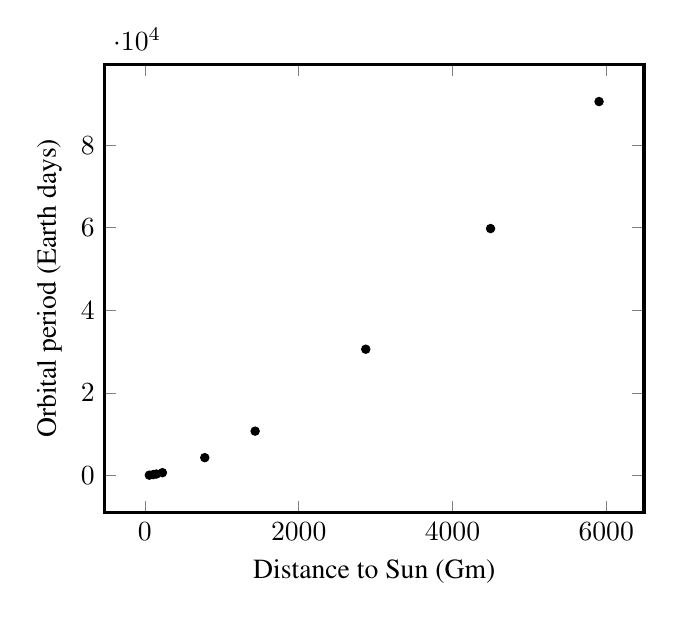
\begin{tikzpicture}
\tikzset{%%
  every mark/.append style={scale=1.0},%%
  scale=1.0%%
}
\pgfplotsset{%%
  every axis/.append style={font=\normalsize}%%
}
%%
\begin{axis}[%%
  axis line style=very thick,%%
  dotStyle/.style={mark size=1.5,black,mark color=black,mark=*,only marks},%%
  enlargelimits=true,%%
  %% x axis
  xlabel={\normalsize Distance to Sun~(Gm)},%%
  xtick={0,2000,4000,6000},%%
  xticklabels={$0$,$2000$,$4000$,$6000$},%%
  %% y axis
  ylabel={\normalsize Orbital period~(Earth days)}%%
]
%%
%%
\addplot[dotStyle] coordinates {
  (57.9, 88)
  (108.2, 224.7)
  (149.6, 365.2)
  (227.9, 687)
  (778.6, 4331)
  (1433.5, 10747)
  (2872.5, 30589)
  (4495.4, 59800)
  (5906.4, 90560)
};
\end{axis}
\end{tikzpicture}

\end{document}
